\pagebreak
\section{Model evaluation results}

Correlation 

\begin{figure}[ht]
    \centering
    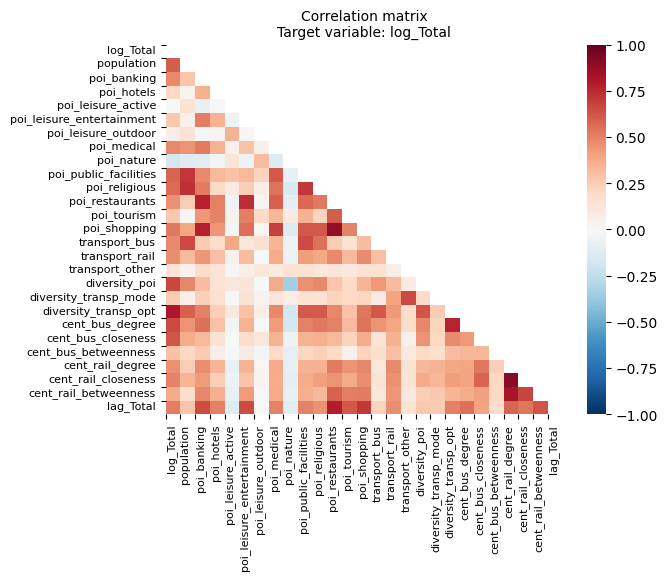
\includegraphics[width=0.8\textwidth]{correlation.png}
    \caption{Correlation matrix of the input features and target variable Total arivals (log)}
    \label{fig:corrmatt}
\end{figure}


Compare

\begin{table}[ht]
    \centering
    \renewcommand{\arraystretch}{1.5}
    \begin{tabular}{|c|c|c|}
        \hline
        \rowcolor{lightgray}
        \textbf{Model} & \textbf{$R^2$ (raw)} & \textbf{$R^2$ (log)} \\
        \hline
        Linear Regression & 0.576 & 0.697 \\
        \rowcolor{pink}
        XGBoost & 0.633 & \textbf{0.792} \\
        ANN & 0.526 & 0.410\\
        \hline
    \end{tabular}
    \caption{Model evaluation results}
    \label{tab:modeleval}
\end{table}

XGBoost chosen becauase blah blah.
Finetuned XGBoost

\begin{table}[ht]
    \centering
    \renewcommand{\arraystretch}{1.5}
    \begin{tabular}{|c|c|c|c|}
        \hline
        \rowcolor{lightgray}
        \textbf{Timeband} & \textbf{R$^2$} & \textbf{MSE} & \textbf{MAE} \\
        \hline
        Total   & \textbf{0.823} & 0.687 & 0.570 \\
        Morning & \textbf{0.809} & 0.614 & 0.571 \\
        Midday  & \textbf{0.828} & 0.629 & 0.549 \\
        Evening & \textbf{0.819} & 0.687 & 0.593 \\
        Late    & \textbf{0.824} & 0.635 & 0.601 \\
        \hline
    \end{tabular}
    \caption{Fine-tuned XGBoost model evaluation results for all target variables}
    \label{tab:modelevaltimeband}
\end{table}

Outlier

\begin{figure}[ht]
    \centering
    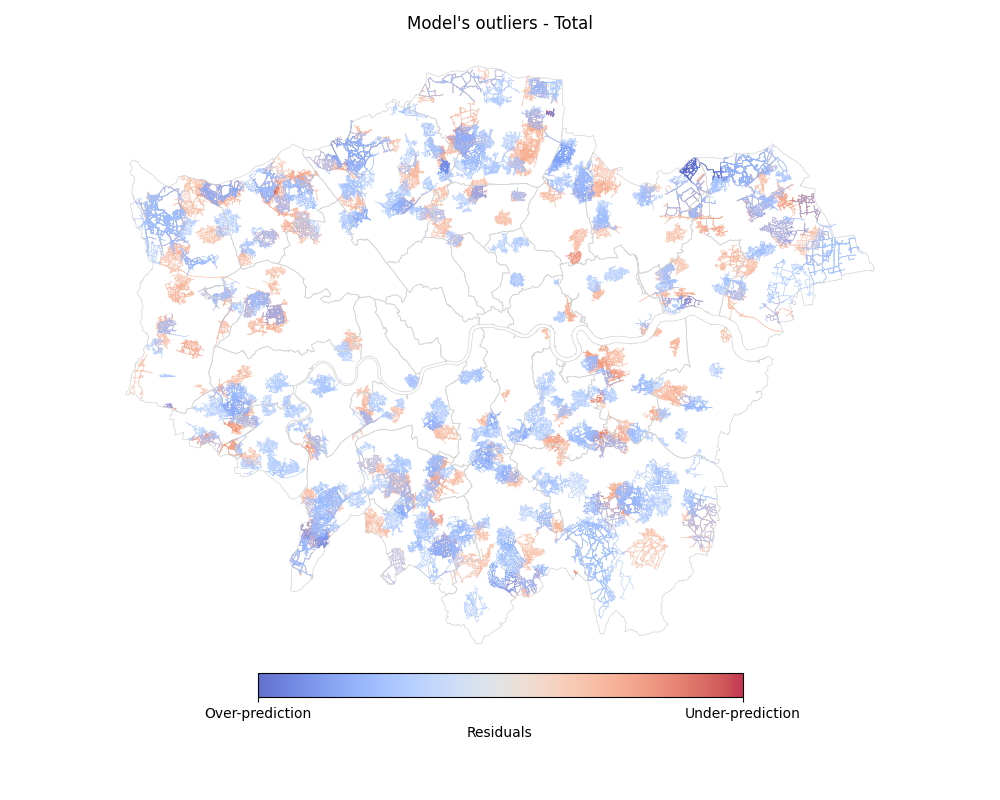
\includegraphics[width=0.8\textwidth]{outliers.png}
    \captionsetup{justification=centering}
    \caption{Outlier spatial units (N=576)\\Fine-tuned XGBoost model predicting Total arrivals (log)}
    \label{fig:outliers}
\end{figure}

Outlier breakdown

\begin{figure}[ht]
    \centering
    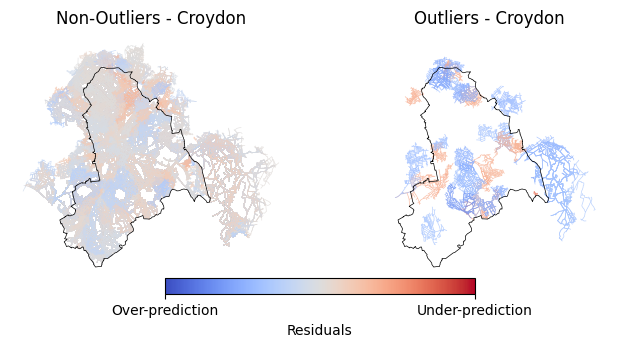
\includegraphics[width=0.8\textwidth]{outliercroydon.png}
    \captionsetup{justification=centering}
    \caption{Profile in model prediction outliers in Croydon}
    \label{fig:outliercroydon}
\end{figure}


\section{Global feature importance}

Global feature importance

\begin{figure}[!ht]
    \centering
    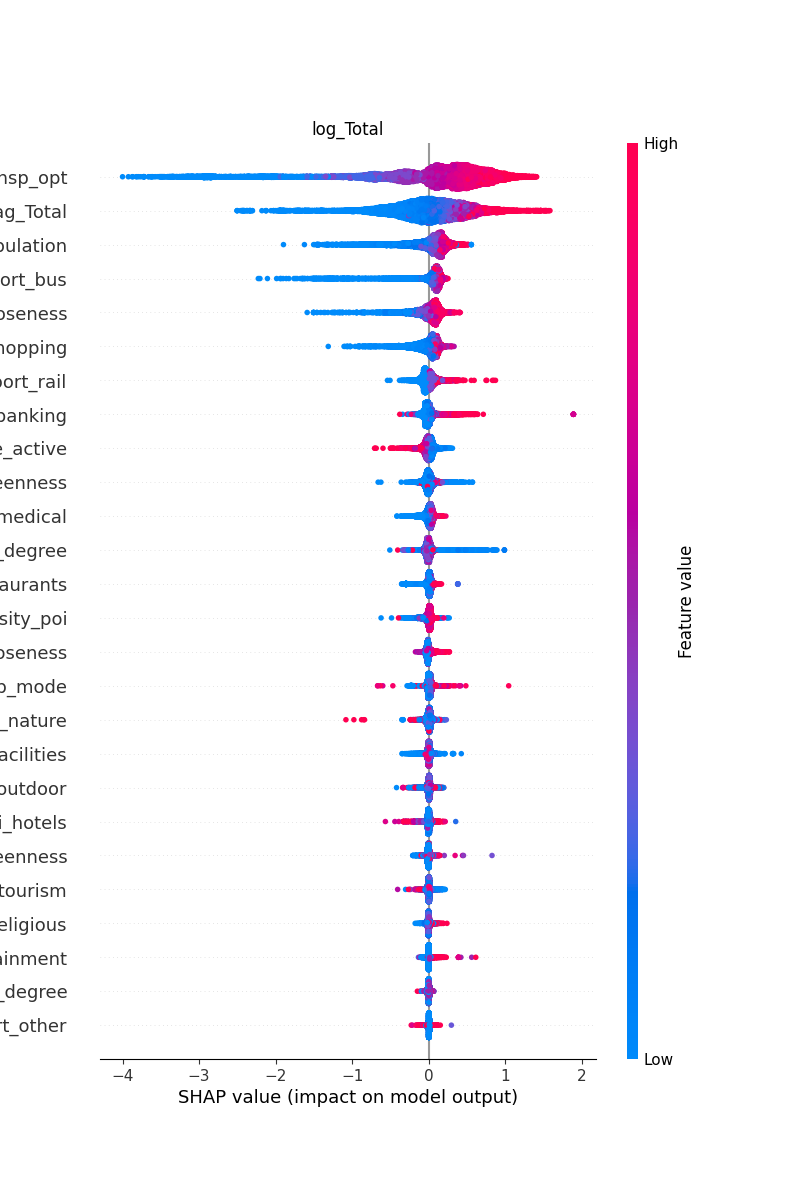
\includegraphics[width=0.8\textwidth]{beeswarm_log_Total.png}
    \captionsetup{justification=centering}
    \caption{Summary of feature importance and partial dependence\\Total arrivals (log)}
    \label{fig:beeswarmtotal}
\end{figure}

\begin{figure}[!ht]
    \centering
    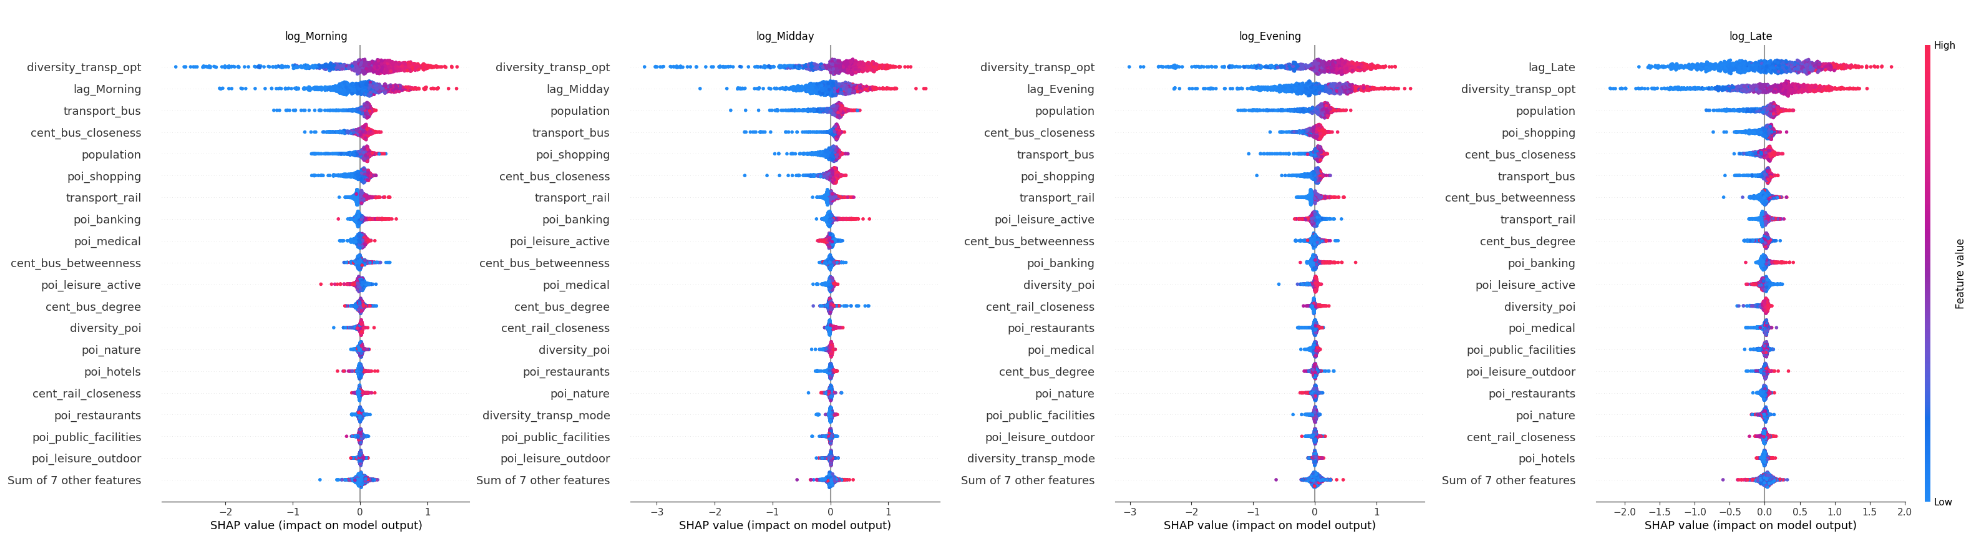
\includegraphics[width=\textwidth]{summarytimeband.png}
    \captionsetup{justification=centering}
    \caption{Summary of feature importance and partial dependence\\By time band (log)}
    \label{fig:beeswarmtimeband}
\end{figure}

\begin{figure}[!ht]
    \centering
    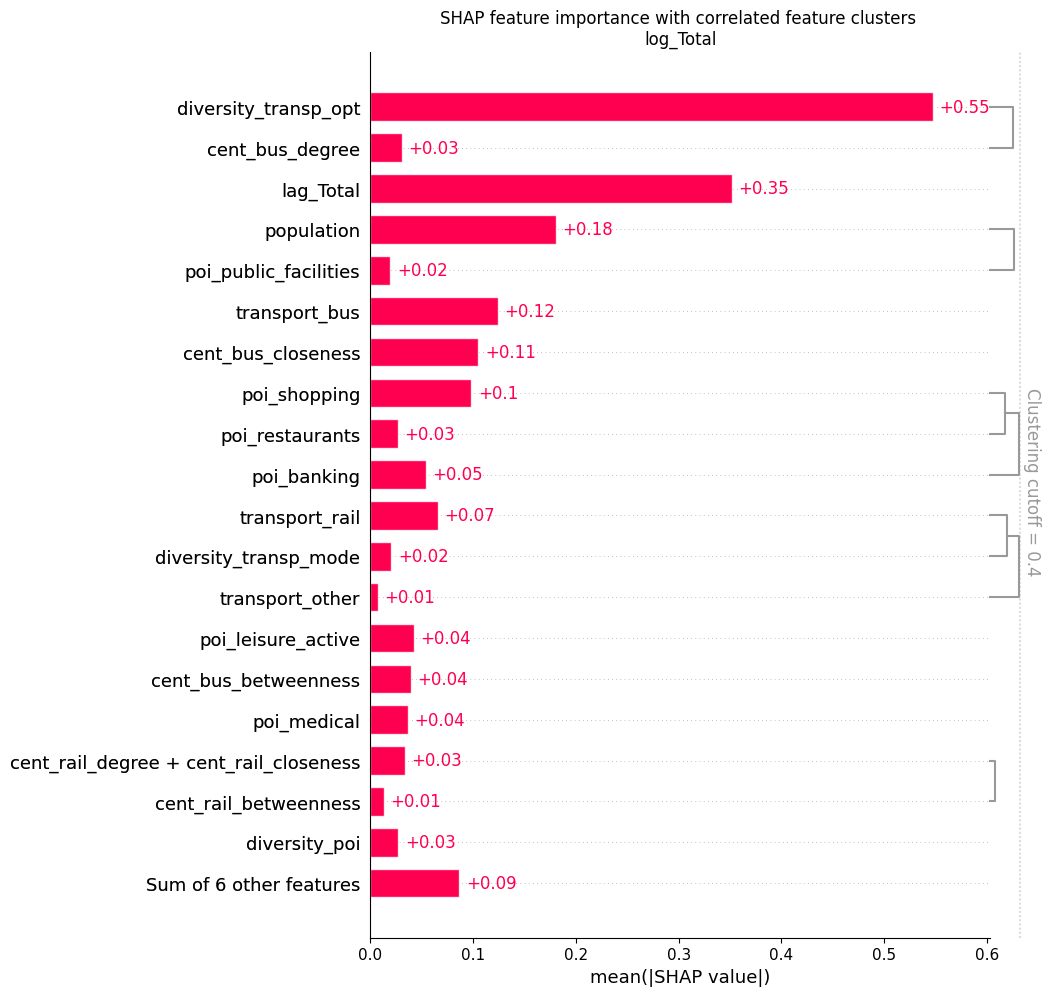
\includegraphics[width=0.8\textwidth]{new_barclus_log_Total.png}
    \captionsetup{justification=centering}
    \caption{Feature importance in predicting Total arrivals (log) \\ (Features clustered by correlation)}
    \label{fig:barclustertotal}
\end{figure}

\begin{figure}[!ht]
    \centering
    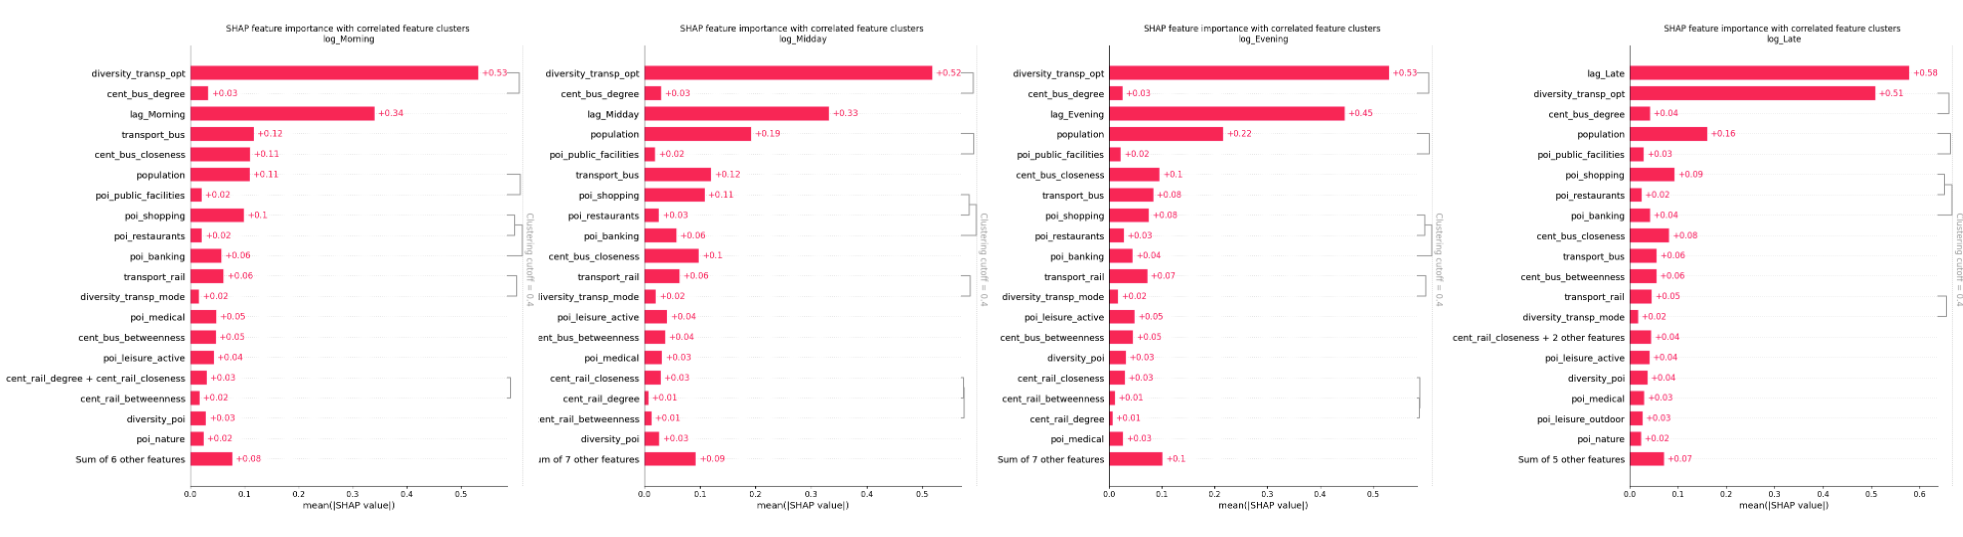
\includegraphics[width=\textwidth]{barclustimeband.png}
    \captionsetup{justification=centering}
    \caption{Feature importance in predicting Arrivals by time band (log) \\ (Features clustered by correlation)}
    \label{fig:barclustertimeband}
\end{figure}

\section{Local feature importance}

Local feature importance

\begin{figure}[!ht]
    \centering
    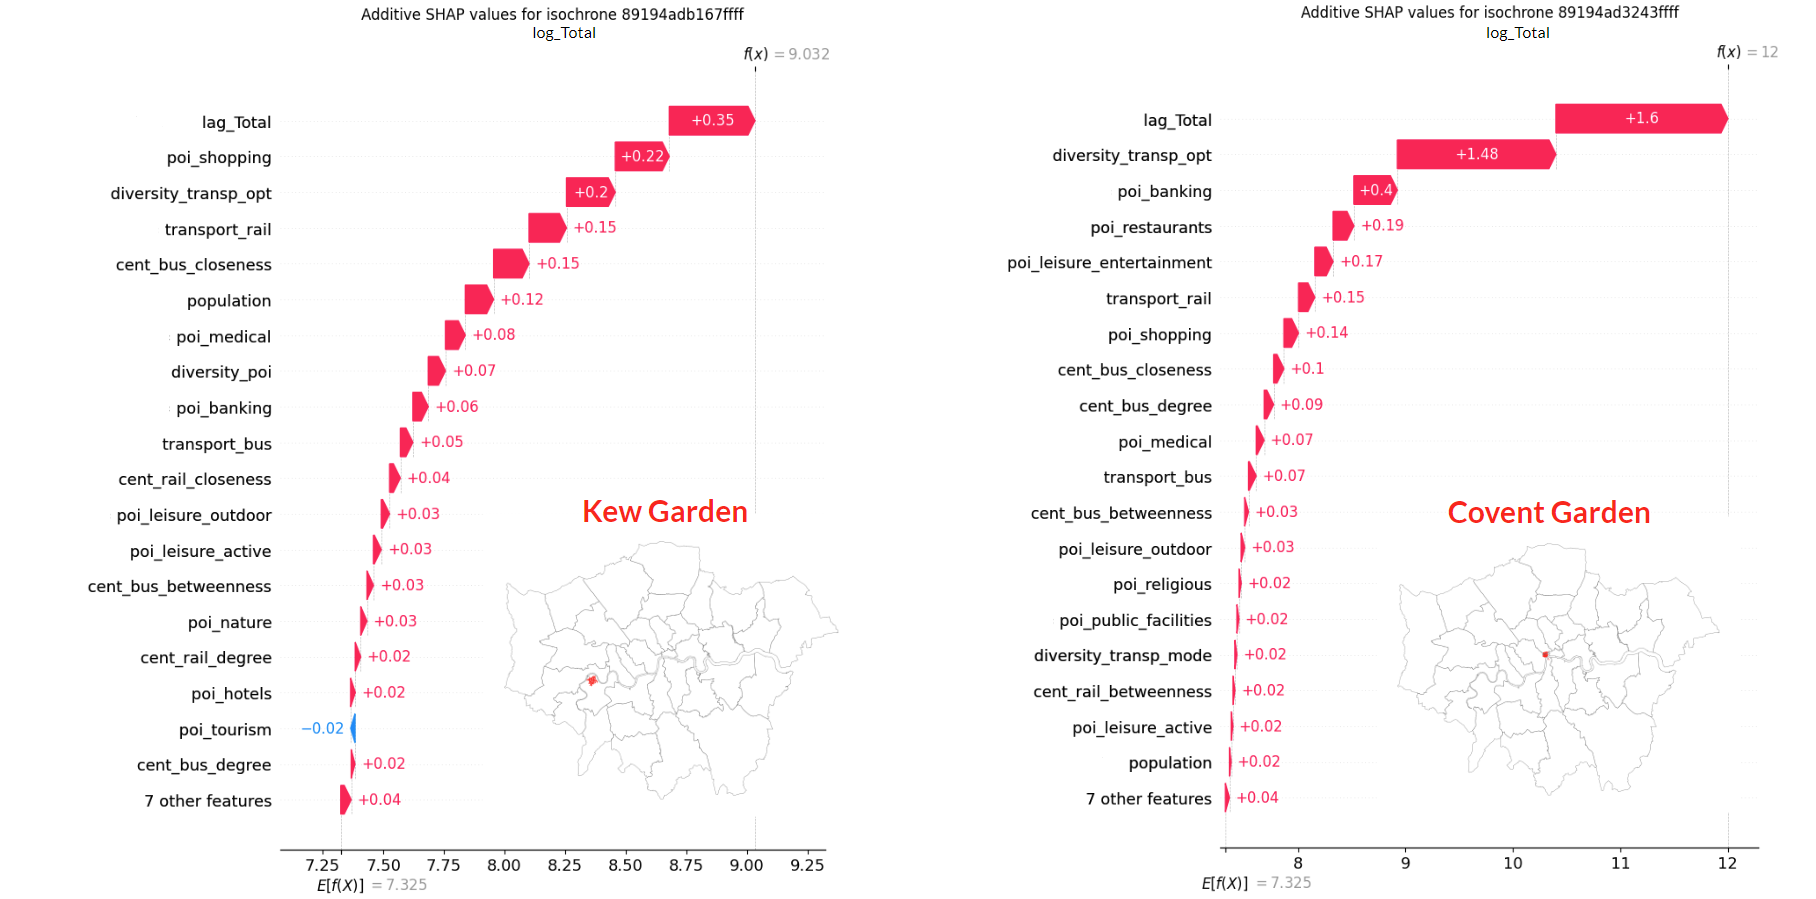
\includegraphics[width=\textwidth]{localshap.png}
    \captionsetup{justification=centering}
    \caption{Local SHAP values for 2 spatial units\\Kew Gardens and Covent Garden}
    \label{fig:localshap}
\end{figure}




\section{Hot spots}

Hot spots for features

\begin{figure}[!ht]
    \centering
    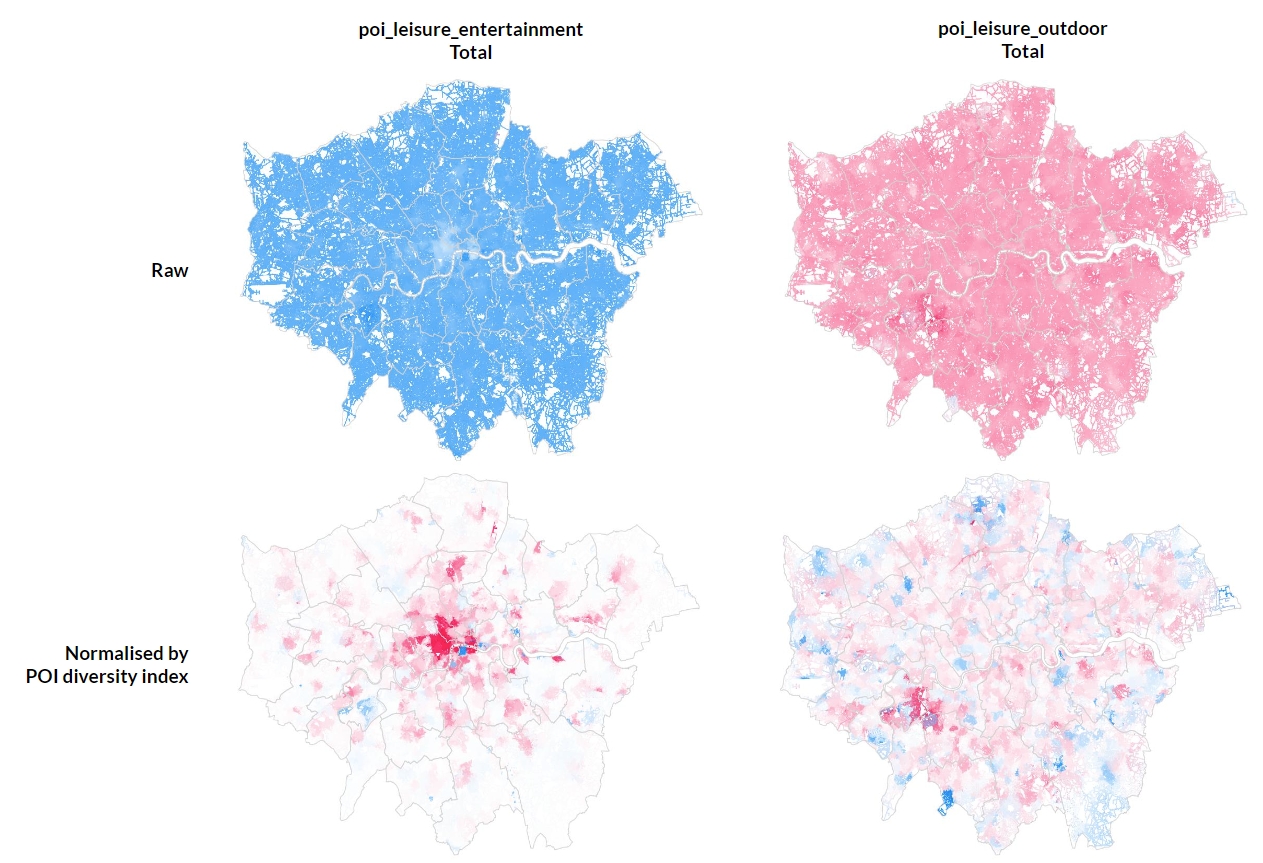
\includegraphics[width=\textwidth]{shaprawweighted.png}
    \captionsetup{justification=centering}
    \caption{Raw vs. weighted SHAP for 2 features\\Outdoor leisure POIs and Entertainment leisure POIs \\Total arrivals (log)}
    \label{fig:shaprawweighted}
\end{figure}


\begin{figure}[!ht]
    \centering
    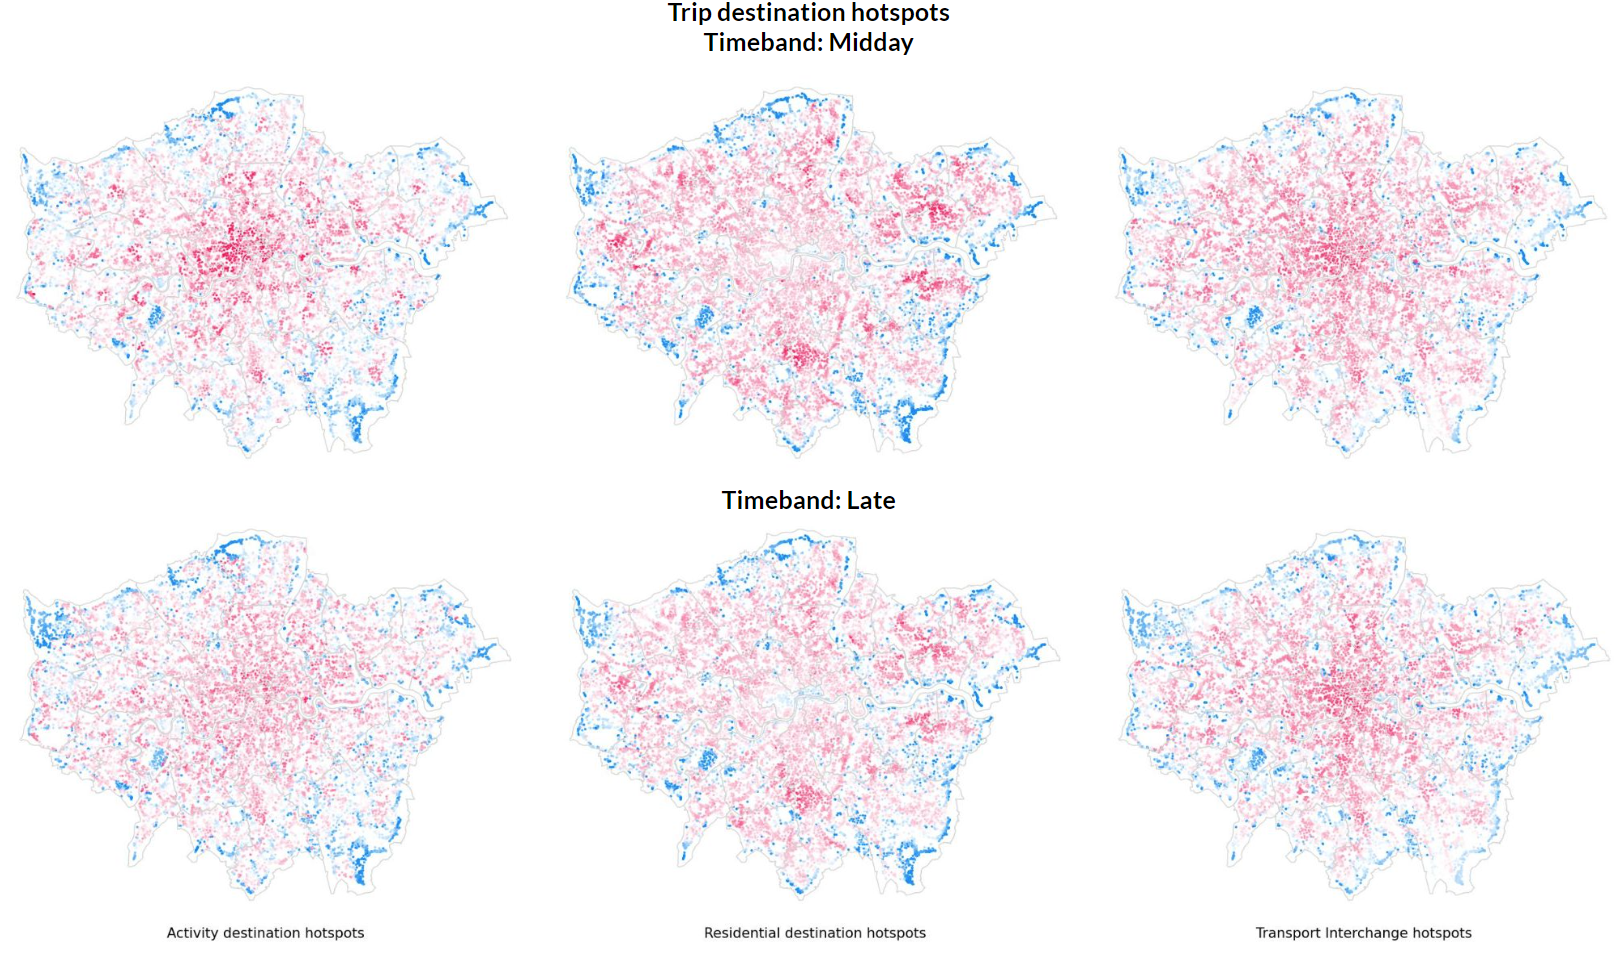
\includegraphics[width=0.75\textwidth]{shaprawweightedmiddaylate.png}
    \captionsetup{justification=centering}
    \caption{}
    \label{fig:shaprawweightedtimeband}
\end{figure}

Hot spots for groups of activities by time band

\begin{figure}[!ht]
    \centering
    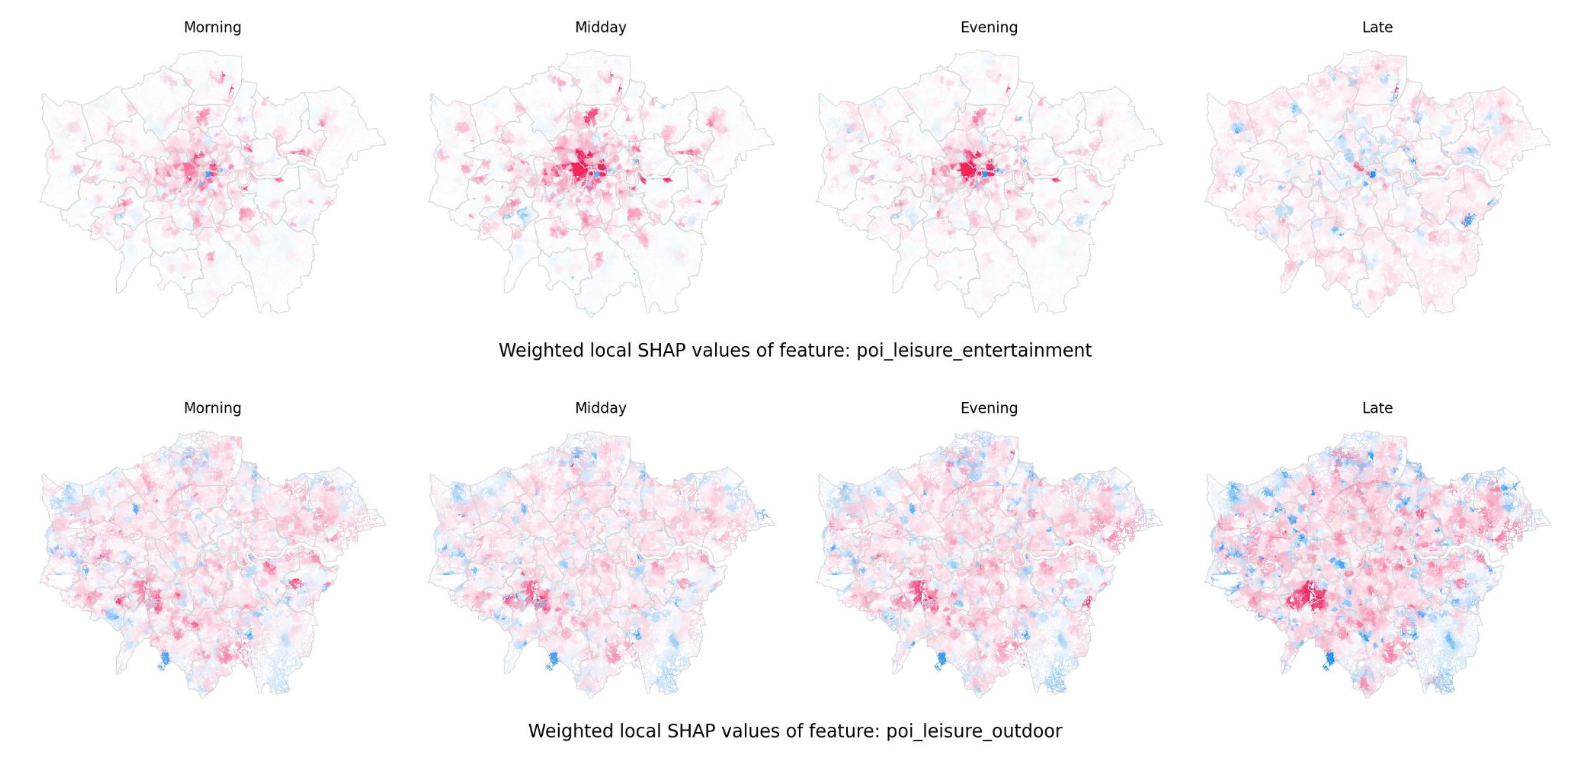
\includegraphics[width=\textwidth]{hotspotstimeband.png}
    \captionsetup{justification=centering}
    \caption{Hot spots\\Arrivals by time band (log)}
    \label{fig:hotspottimeband}
\end{figure}


\section{Discussions}

\subsection{Implications on urban analytics literature}

\subsection{Implications on transport planning}

\subsection{Limitations and future work}